%%%%%%%%%%%%%%%%%%%%%%%%%%%%%%%
%   Figures for chapter 5
%%%%%%%%%%%%%%%%%%%%%%%%%%%%%%%

\newcommand{\figSupportedAgents}{
    \begin{figure}[!ht]
        \centering
        \begin{subfigure}[b]{0.3\textwidth}
            \centering
            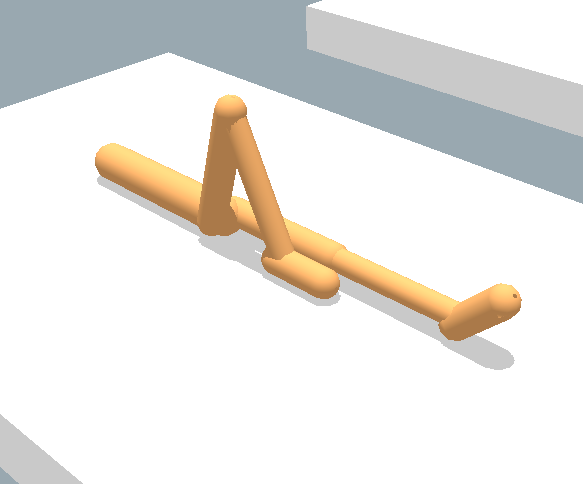
\includegraphics[width=0.9\textwidth]{./chapters/chapter_5/imgs/img_ch5_agents_controlsuite_walker.png}
            \caption{}
        \end{subfigure}
        \begin{subfigure}[b]{0.3\textwidth}
            \centering
            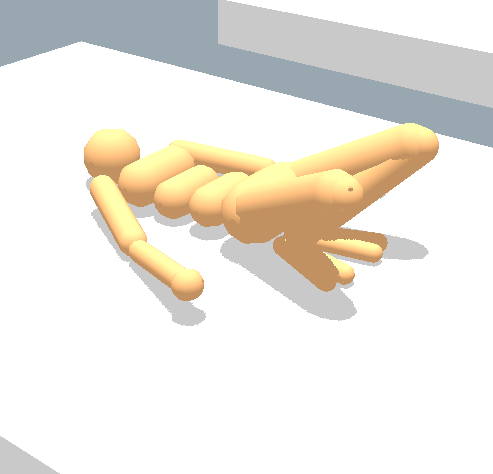
\includegraphics[width=0.9\textwidth]{./chapters/chapter_5/imgs/img_ch5_agents_controlsuite_humanoid.png}
            \caption{}
        \end{subfigure}
        \begin{subfigure}[b]{0.3\textwidth}
            \centering
            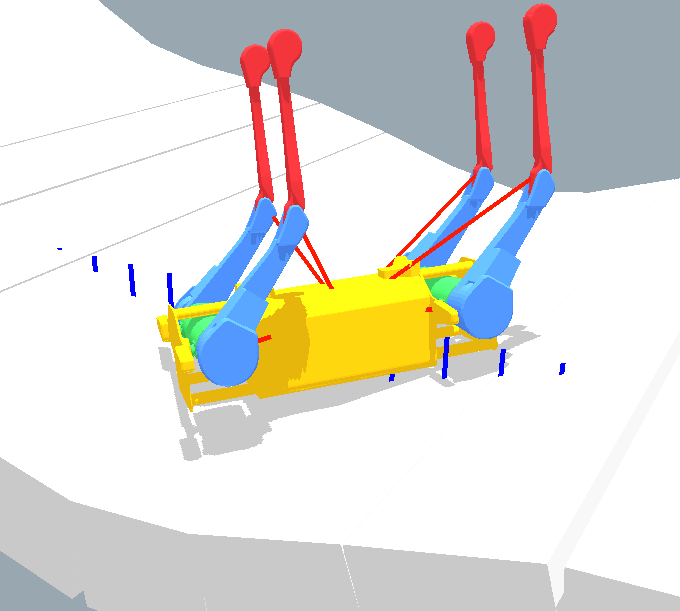
\includegraphics[width=0.9\textwidth]{./chapters/chapter_5/imgs/img_ch5_agents_pybullet_laikago.png}
            \caption{}
        \end{subfigure}
        \caption{Current agents supported in the framework. Walker (a) and humanoid (b) 
                 from \citeauthor{Controlsuite}, and laikago (c) from \citeauthor{PyBullet}.}
        \label{fig:ch5_current_supported_agents}
    \end{figure}
}


\newcommand{\figProgressAgents}{
    \begin{figure}
        \centering
        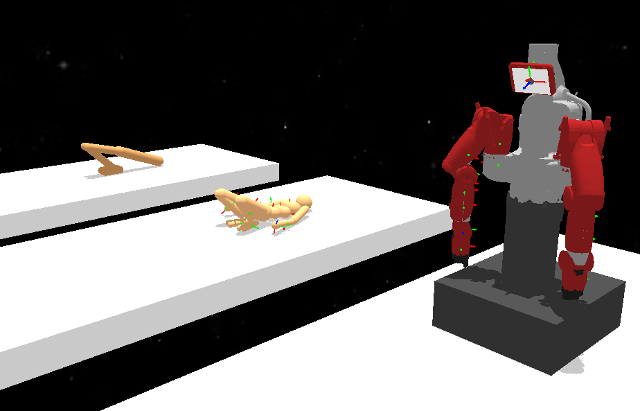
\includegraphics[width=0.9\textwidth]{./chapters/chapter_5/imgs/img_tysocmjc_agents.png}
        \caption{Current agent support. Refer to \href{https://youtu.be/5zv5SK0o92I}{this}
                 video for a test of the current functionality.}
        \label{fig:ch5_progress_agents}
    \end{figure}
}

\newcommand{\figProgressSensors}{
    \begin{figure}
        \centering
        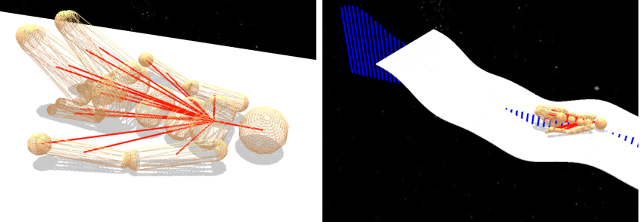
\includegraphics[width=0.9\textwidth]{./chapters/chapter_5/imgs/img_tysocmjc_sensors.png}
        \caption{Current sensor support. Currently the framework supports: 
                            a) intrinsic measurements (joint angles and velocities, body velocities and acceelrations, and relative positions).
                            b) extrinsic measurements (height fields taken from the terrain)}
        \label{fig:ch5_progress_sensors}
    \end{figure}
}

\newcommand{\figProgressTerrains}{
    \begin{figure}
        \centering
        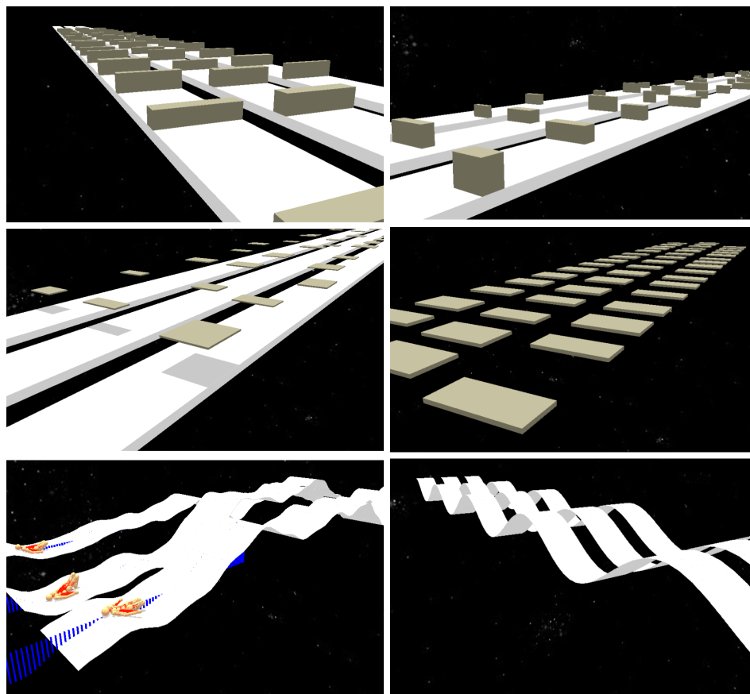
\includegraphics[width=0.9\textwidth]{./chapters/chapter_5/imgs/img_tysocmjc_terrains.png}
        \caption{Current terrain support. Currently the framework supports the
                 environments from \citeauthor{DeepmindEmergenceLocomotion}}
        \label{fig:ch5_progress_terrain}
    \end{figure}
}